\chapter{SCEPTIC3DGPU Validation}

To validate the GPU version of SCEPTIC3D we compared the diagnostic outputs of the two codes and ensured that the relative error was small. SCEPTIC3D's typical terminal output is shown in figure \ref{fig:term_output}. All of the following runs were performed using 42 million particles on a $64^3$ grid and run for 200 steps. 

\begin{figure}
\begin{lstlisting}[frame=single]
Mesh:  64 x 64 x 64  Particles:42000000 Bz:  1.25
l_d=0.500 Ti=0.100 Steps=200 dt=0.0250 rmax=10.0 vd=0.500 vp=-4.0000
reinjFrac= 0.279223
Probe flux density=  0.8862
Probe energy flux= 43.4997
   z E-field   z Electrons   z Ions     z Lorentz    z Total    Charge
  -10.813281    0.000000   13.668346    0.000000   10.965026  -98.108620
   -0.007198    7.090378    8.079660    0.000000   15.168240   -9.301228
 
   x E-field   x Electrons   x Ions     x Lorentz    x Total
    0.442024    0.000000   -0.048813    0.000000    0.061692
    0.003924   -0.235518   -0.035265    0.000000   -0.269802
 
   y E-field   y Electrons   y Ions     y Lorentz    y Total
    0.247737    0.000000   -0.036909    0.000000    0.025025
    0.003151   -0.122853    0.023184    0.000000   -0.098881
 rhoinf   10446.92    
 Outer potential -8.3603784E-03
Ion Forces: Inner, outer, uncertainty,   13.6683    8.0797+- 0.0564
 Time :    3100.83495712280    
\end{lstlisting}
\vspace{-0.4in}
\caption{Typical terminal ouputs from SCEPTIC3D.}
\label{fig:term_output}
\end{figure}

The GPU and CPU code will not give the same values for several reasons, despite GPUs having IEEE-754 mathematical operations. First, x86 processors lack the fused multiply add (FMAD) instruction that is used on the GPU. Normal x86 multiple-add procedure is to perform the multiply, round, add, round. The FMAD instruction skips the round after the multiply and instead carries an extra bit of precision from the multiply into the add. The only rounding operation performed in the FMAD instruction is after the add. \cite{Whitehead2011}

The second reason for differences in output is the nature of the parallel operations used to total data on the GPU, and the undefined nature of atomic operations. Sums calculated using parallel prefix sum are added up in a different order than those calculated by a serial summation.\cite{Whitehead2011} The same is true for atomic operations since the order of operations with atomic operations is not defined. This also leads to a situation where no two GPU runs will return exactly the same answer, even if the initial conditions are exactly the same from run to run.\cite{NVIDIACorporation2011}

Figures \ref{fig:gpu_validation_pflux} and \ref{fig:gpu_validation_density} show side-by-side two of SCEPTIC3D's final outputs. Judging from the figures, the GPU code output is the essentially the same as the CPU output. A more quantitative comparison can be seen in table \ref{tab:cpu_gpu_data_compare}. We can isolate the uncertainty induced by the order of the atomic operations by comparing multiple runs of the GPU code. These results are shown in table \ref{tab:gpu_gpu_data_compare}. 


\begin{figure}
\centering
\noindent
	\subfloat[CPU Output]{
		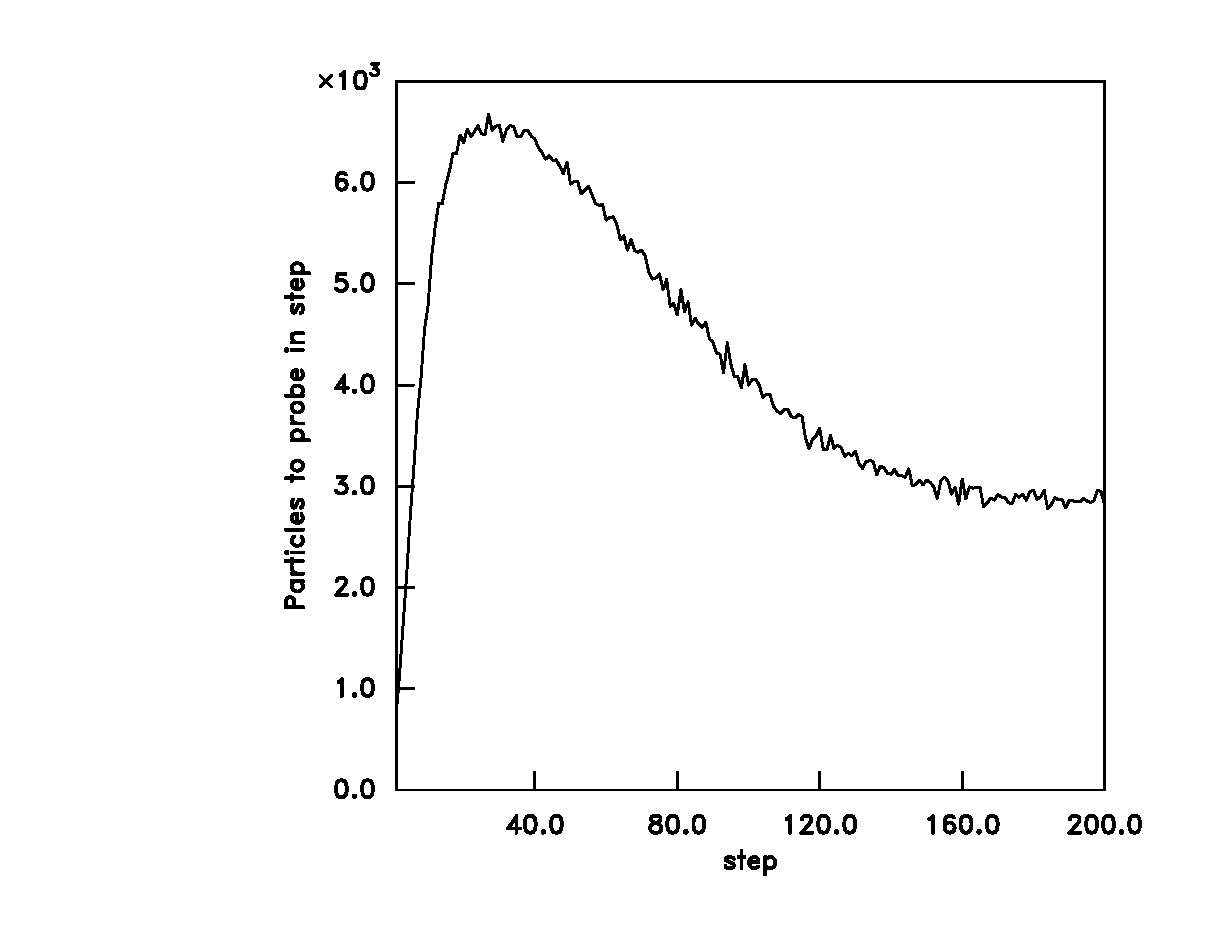
\includegraphics[viewport=1.75in 0 8.19in 6.25in,width=3.0in,clip]{./appa/plot0001_cpu.pdf}}
	\subfloat[GPU Output]{
		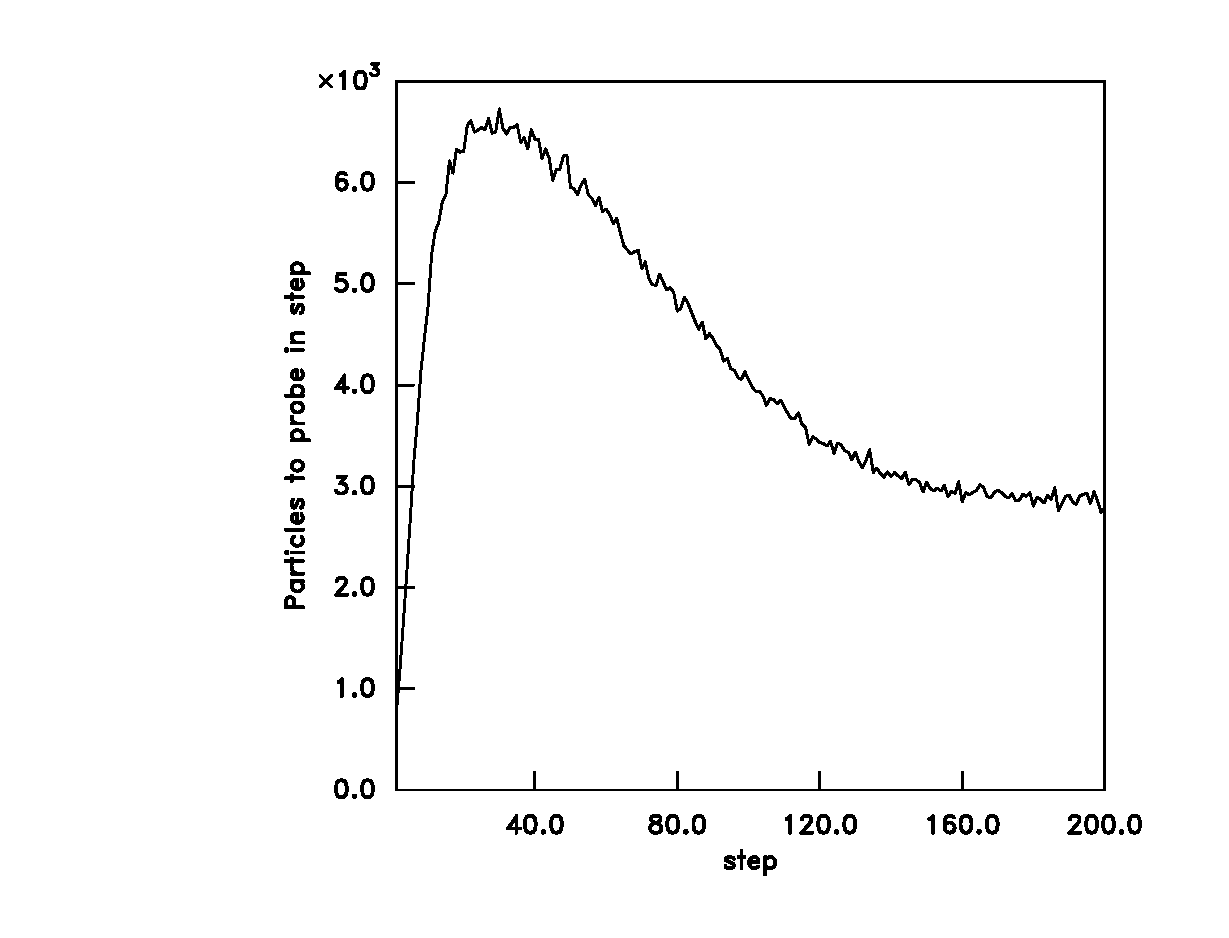
\includegraphics[viewport=1.75in 0 8.19in 6.25in,width=3.0in,clip]{./appa/plot0001_gpu.pdf}}
	\caption[GPU Validation: Particle Flux Comparison]{Comparison of particle flux to probe calculated by the CPU version and GPU version of SCEPTIC3D}	
	\label{fig:gpu_validation_pflux}
\end{figure}

\begin{figure}
\centering
\noindent
	\subfloat[CPU Output]{
		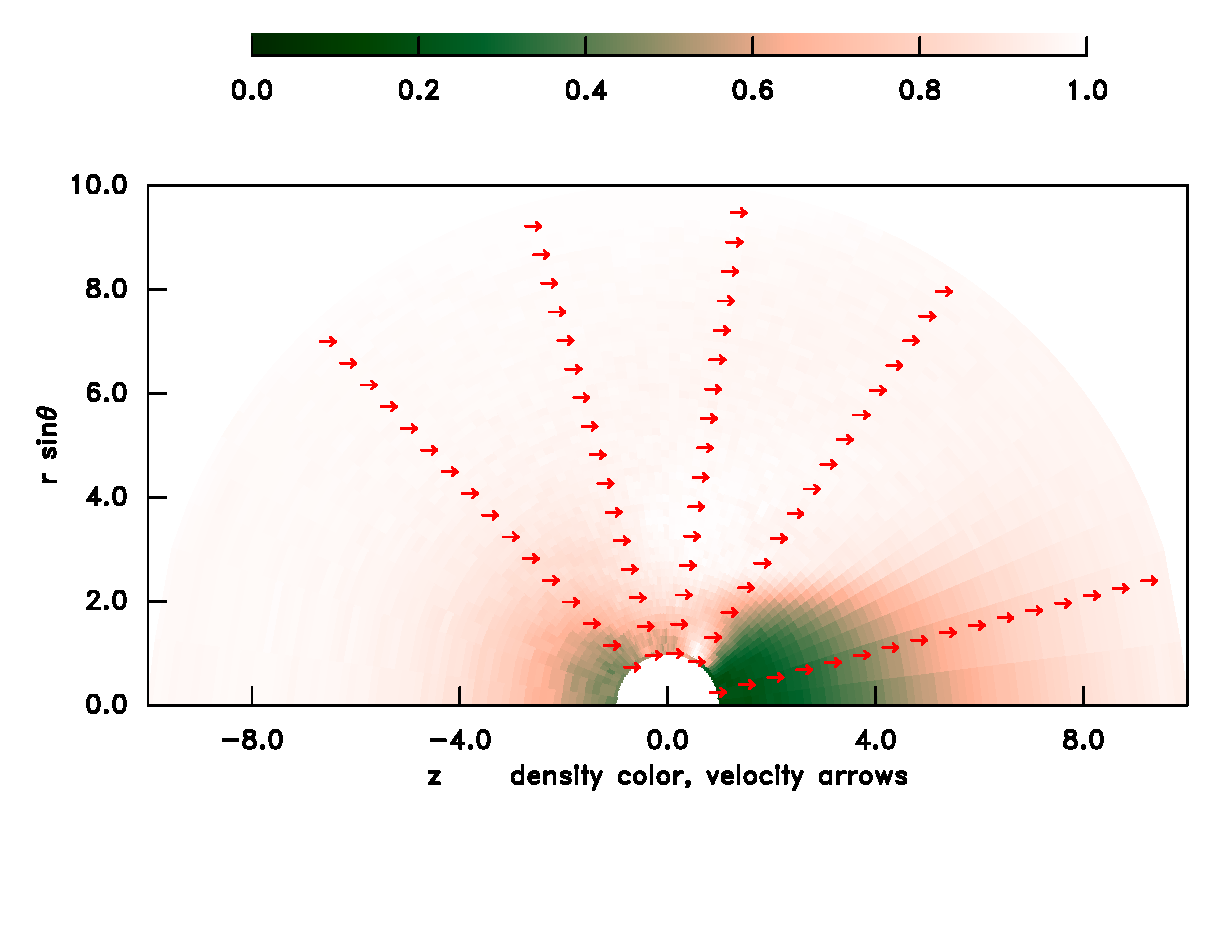
\includegraphics[width=3.0in]{./appa/plot0002_cpu.pdf}}
	\subfloat[GPU Output]{
		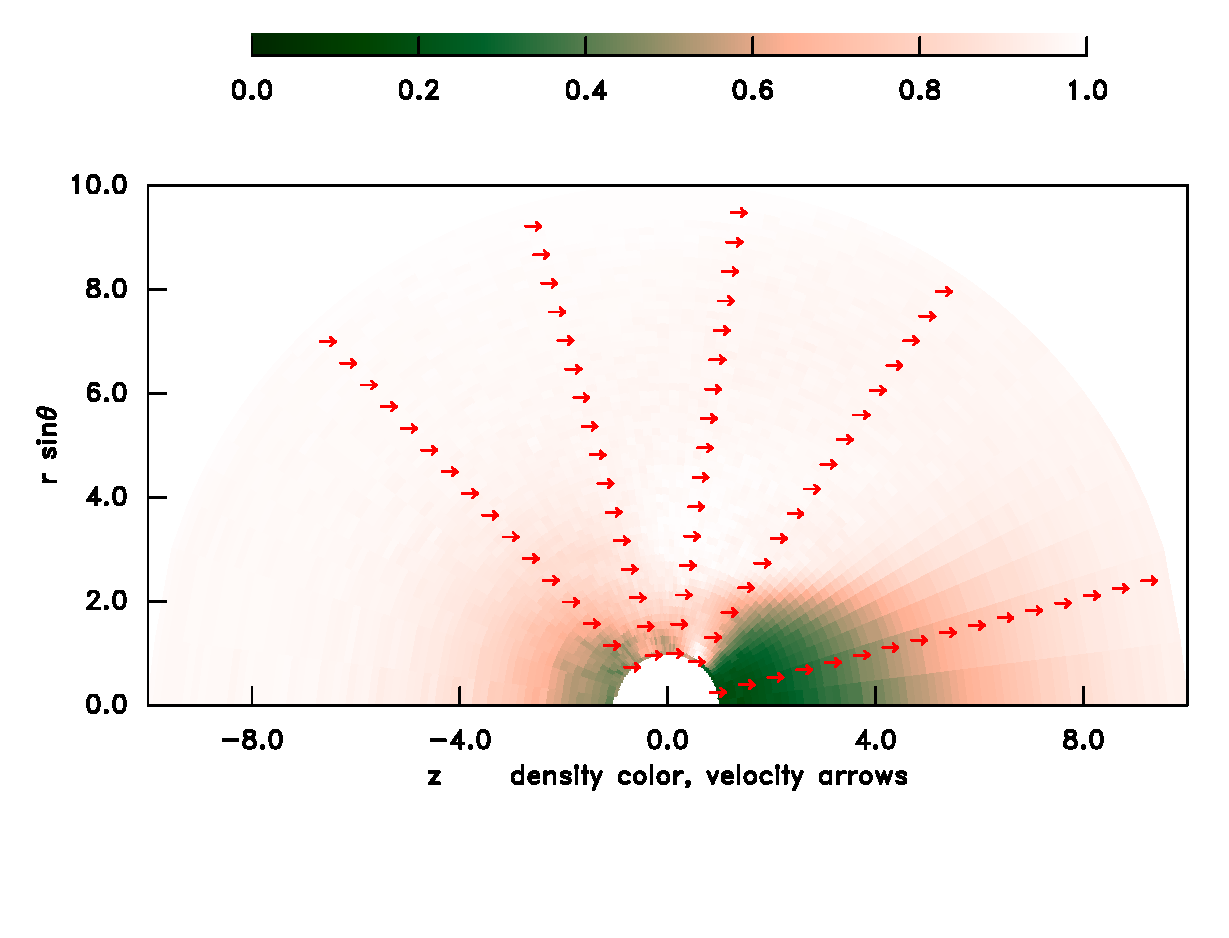
\includegraphics[width=3.0in]{./appa/plot0002_gpu.pdf}}
	\caption[GPU Validation: Particle Flux Comparison]{Comparison of density calculated by the CPU version and GPU version of SCEPTIC3D. Velocity output disabled as it has not been implemented in the GPU code yet.}	
	\label{fig:gpu_validation_density}
\end{figure}



\begin{table}
\begin{tabular}{| p{4.0cm} | p{3.5cm} | p{2.5cm} | p{4.0cm} |}
\hline
Output 						& CPU Value 		& GPU Value 		& Relative Error \\ \hline
Probe flux density 		& 0.8862 			& 0.8861 			& 1.1285e-4 \\ \hline
Probe energy flux   		& 43.4997 			& 43.4977 			& 4.5978e-5 \\ \hline
Charge 						& -98.10862 		& -98.108398 		& 2.2628e-6 \\ \hline
Rho Infinity 				& 10446.92 			& 10447.37 			& 4.3074e-5 \\ \hline
Outer Potential 			& -8.3604e-3 		& 8.3241e-3 		& 4.3458e-3 \\ \hline
Inner Ion Force 			& 13.6683 			& 13.6677 			& 4.3898e-5 \\ \hline
Outer Ion Force 			& 8.0797 			& 8.0856 			& 7.2996e-4 \\ \hline
Ion Force Uncertainty 	& 0.0564 			& 0.0556 			& 1.4286e-2 \\ \hline
Fraction Reinjection 	& 0.279179			& 0.279187 			& 5.5131e-4 \\ \hline
\end{tabular}
\caption[CPU and GPU SCEPTIC3D Output Comparison]{Comparison of common SCEPTIC3D outputs. The relative error is on the order of that expected for single precision rounding errors and particle noise.}
\label{tab:cpu_gpu_data_compare} 
\end{table}

\begin{table}
\begin{tabular}{| p{4.0cm} | p{3.5cm} | p{2.5cm} | p{4.0cm} |}
\hline
Output 						& GPU Run 1 Values 		& GPU Run 2 Values 		& Relative Error \\ \hline
Probe flux density 		& 0.8862 			& 0.8861 			& 1.1285e-4 \\ \hline
Probe energy flux   		& 43.4985 			& 43.4977 			& 1.8392e-5 \\ \hline
Charge 						& -98.108459 		& -98.108398 		& 6.2176e-7 \\ \hline
Rho Infinity 				& 10447.1 			& 10447.37 			& 2.5844e-5 \\ \hline
Outer Potential 			& -8.3265e-3 		& 8.3241e-3 		& 2.8828e-4 \\ \hline
Inner Ion Force 			& 13.6680 			& 13.6677 			& 2.1949e-5 \\ \hline
Outer Ion Force 			& 8.0860	 			& 8.0856 			& 4.9469e-5 \\ \hline
Ion Force Uncertainty 	& 0.0561 			& 0.0556 			& 8.9526e-3 \\ \hline
Fraction Reinjection 	& 0.279188			& 0.279187 			& 3.5818e-6 \\ \hline
\end{tabular}
\caption[GPU SCEPTIC3D Output Comparison for 2 GPU runs]{Comparison of common SCEPTIC3D outputs for multiple GPU runs. These errors are roughly 1 to 2 times larger than the difference between the CPU and the GPU outputs.}
\label{tab:gpu_gpu_data_compare} 
\end{table}


\clearpage
\newpage





